\vspace{-12pt}
\section{Replicating SDR}
\vspace{-8pt}


%\subsection{Observations on Relevant Documents}
In the original paper of Lee and Sun, they devise two experimental settings for SDR: an initial ranking of retrieved studies using a seed study and iteratively re-ranking by updating the query used for SDR with one seed study at a time to simulate the manual screening process. We focus on the initial ranking stage for two reasons: (1) screening prioritisation is an accepted practice in the systematic review creation process as all studies must still be screened~\cite{chandler2019cochrane}; and (2) an effective initial ranking will naturally result in a more effective and efficient re-ranking of studies, as more studies that are relevant will be identified faster.
The intuition for SDR is that relevant studies are similar to each other. The original paper makes two important observations about seed studies to support this intuition: (1) that relevant studies are more similar to each other than they are to non-relevant studies; and (2) that relevant studies share many \textit{clinical terms}. These two observations are used to inform the representation and scoring of studies, given a seed study. We attempt to replicate these observations below to verify both that our implementation follows the same steps to make similar observations and whether the assumptions derived from them hold.
%
%We begin by investigating these observations about clinical terms to determine if the intuitions about using them are valid or not.

\begin{observation}
For a given systematic review, its relevant documents share higher pair-wise similarity than that of irrelevant documents.
\end{observation}

%The observation made is valid as relevant studies do share higher intra similarity compared with irrelevant documents. However, as negative studies were randomly chosen, the differences between their actual differences can only be treated as a reference, the actual comparing space for negative studies are much larger than that of positive studies, which means, higher intra-similarities with a particular seed document would always represent the study will be included definitely.
\noindent
We find that this observation is valid in our reproduction, as demonstrated by Figure~\ref{fig:replicating.pairwise-similarity}. In order to produce this plot, irrelevant studies were randomly under-sampled ten times. The number of non-relevant studies is always the same as the number of relevant studies for each topic. This means it is unlikely that we will produce the exact result initially found for this observation by Lee and Sun. Furthermore, one reason that the average pairwise similarity for the relevant studies may not match the original results is that the textual content of studies on PubMed may have changed or been updated. Rather than using a dump of PubMed from 2017, we used the latest version of studies on PubMed, as it is unknown the exact date that studies were extracted from PubMed in the original paper, and the CLEF TAR dataset does not give an exact date. 



\begin{observation}
Relevant documents for a given systematic review share high commonality in terms of clinical terms.
\end{observation}

\noindent
We found that this observation is also valid in our reproduction, as demonstrated in Figure~\ref{fig:replicating.commonality}. It can be seen that the commonality of terms for the bag of words (BOW) and bag of clinical words (BOC) representations closely match those reported by Lee and Sun. However, we also found that with some minor modifications to the pre-processing of studies, we achieved a similar (yet still lower) commonality for terms using the BOW representation. We believe that the BOC representation shares a higher commonality of terms because the vocabulary size is smaller than the BOW representation. 
Naturally, with a smaller vocabulary, it is more likely for studies to share common terms.
%When pre-processing studies using the method suggested in original paper, we obtain a vocabulary size of 1,612,974 from BOW, thus the number of distinct clinical terms extracted only count for 4.6 \% of the vocabulary, while using preprocessing of proposed method in our paper, the number of distinct clinical terms counts for 30 \% in the BOW word space. With thee same number of BOC clinical terms extracted, our method only obtain 14.75 \% of the vocabulary size in original preprocessing method. 
When pre-processing studies using the method described in original paper, we find that BOC terms count for 4.6\% of the vocabulary, while they account for 31.2\% using our pre-processing. In fact, our BOW vocabulary is only 14.8\% their BOW vocabulary. Note that BOC is a distinct subset of BOW.


\begin{figure}[t!]
	\vspace{-12pt}
	\centering
	\begin{minipage}[t]{.48\columnwidth}
		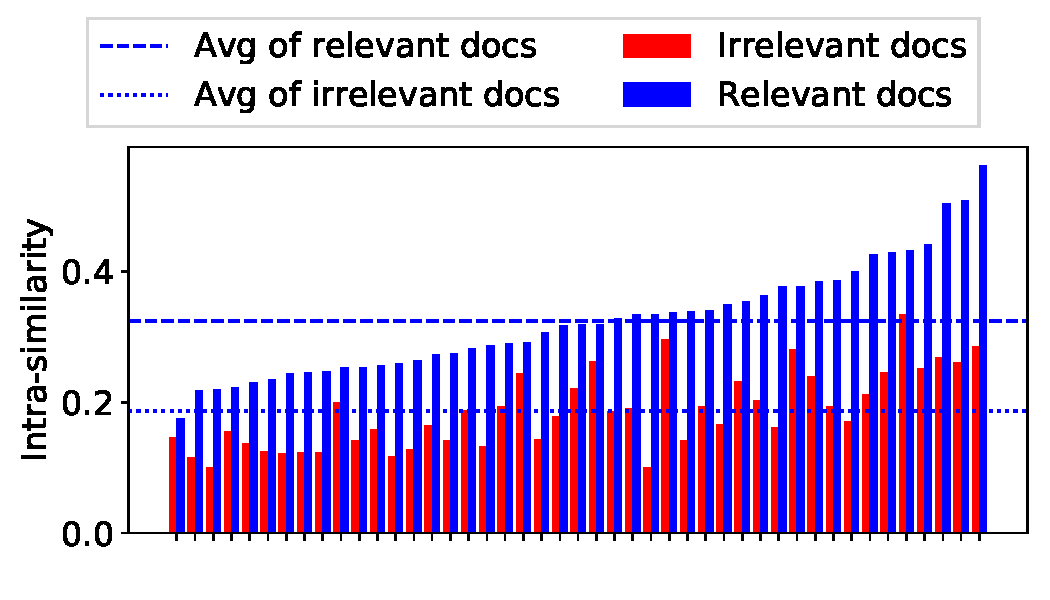
\includegraphics[width=\columnwidth]{pics/intra_sim.pdf}
		\vspace{-24pt}
		\caption{Intra-similarity between relevant studies and irrelevant studies.}
		\label{fig:replicating.pairwise-similarity}
	\end{minipage}
	\hspace{8pt}
	\begin{minipage}[t]{.48\columnwidth}
		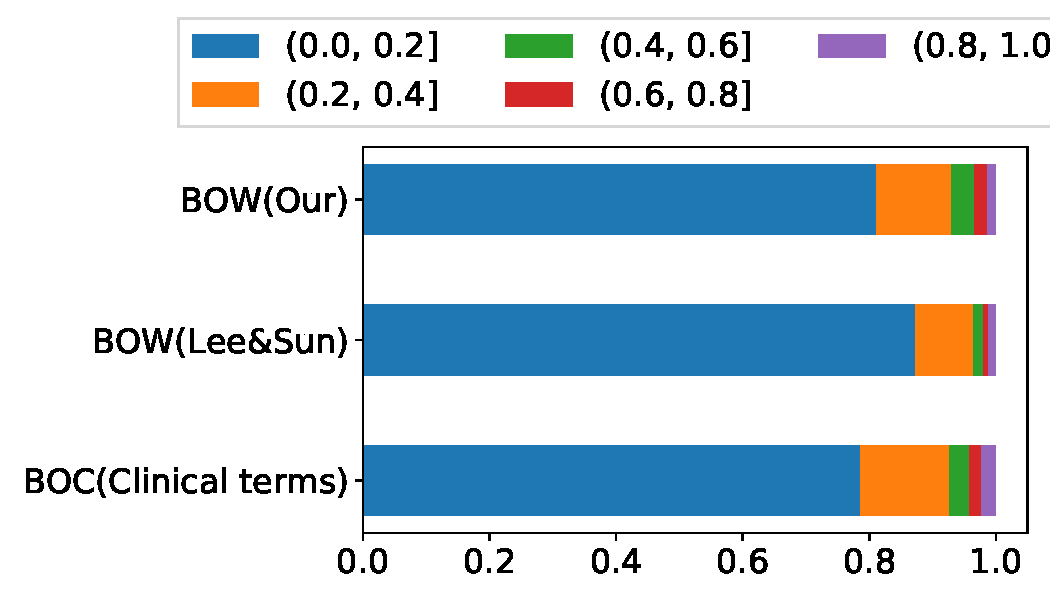
\includegraphics[width=\columnwidth]{pics/weighted1_bow_weighted1_bow_cased_lee_weighted1_boc_word.pdf}
		\vspace{-24pt}
		\caption{Distribution of terms in relevant studies.}
		\label{fig:replicating.commonality}
	\end{minipage}
	\vspace{-12pt}
\end{figure}

\vspace{-12pt}
\subsection{Document Representation}
\vspace{-4pt}

Given Observation 1 about relevant studies for this task, Lee and Sun chose to represent studies as a `bag of clinical words' (BOC). They chose to use the Unified Medical Language System (UMLS) as their ontology of clinical terms. UMLS is an umbrella ontology that combines many common medical ontologies such as SNOMED-CT and MeSH. In order to identify UMLS concepts (and therefore the clinical terms) within the studies, Lee and Sun combine the outputs of the NCBO Bioportal~\cite{noy2009bioportal} API\footnote{\url{http://data.bioontology.org/documentation}} and QuickUMLS~\cite{soldaini2016quickumls}. We follow their process as described, however we are not aware if it is not possible to set a specific version for the NCBO API. We use QuickUMLS version 1.4.0 with UMLS 2016AB.

\vspace{-12pt}
\subsection{Term Weighting}
\label{sec:replicate.term-weighting}
\vspace{-4pt}

SDR weights terms based on the intuition that terms in relevant studies are more similar to each other (or occur with each other more frequently) than non-relevant studies.
%Therefore, SDR weights terms to promote this intuition.
The weight of an individual term in a seed study is estimated by measuring to what extent it separates similar (pseudo-relevant) and dissimilar (pseudo-non-relevant) studies.
Formally, each term $t_i$ in a seed document $d_s$ ($t_i\in d_s$) is weighted using the function $\varphi (t_i,d_s) = \text{ln}\left(1+\frac{\gamma(D_{t_i},d_s)}{\gamma(D_{\bar{t_i}},d_s)}\right)$, 
%in Equation~\ref{eq:term-weight}
%\vspace{-8pt}
%\begin{equation}\label{eq:term-weight}
%	\phi (t_i,d_s) = \text{ln}\left(1+\frac{\gamma(D_{t_i},d_s)}{\gamma(D_{\bar{t_i}},d_s)}\right)
%\end{equation}
%
%\noindent
where $D_{t_i}$ represents the subset of candidate studies to be ranked where $t_i$ appears, and $D_{\bar{t_i}}$ represents the subset of candidate studies to be ranked where $t_i$ does not appear. The average similarity between studies is computed as $\gamma(D, d_s) = \frac{1}{|D|}\sum_{d_j\in D} sim(d_j, d_s)$, 
% in Equation~\ref{eq:similarity}:
%
%\vspace{-8pt}
%\begin{equation}\label{eq:similarity}
%	\gamma(D, d_s) = \frac{1}{|D|}\sum_{d_j\in D} sim(d_j, d_s)
%\end{equation}
%
%\noindent
where $sim$ is the cosine similarity between the vector representations of the candidate study $d_j$ and the seed study $d_i$. 
%In the original implementation, studies were represented as tf-idf vectors. For reproducibility purposes, we use the same representation.
We follow the original implementation and represent studies as tf-idf vectors.

\vspace{-12pt}
\subsection{Document Scoring}
\vspace{-4pt}

The original SDR implementation uses the query likelihood language model with Jelenik-Mercer smoothing for scoring studies. Typically, this ranking function is derived as indicated by QLM shown in Equation~\ref{eq:qlm-jm-sdr}, 
%
%\begin{equation}\label{eq:qlm-jm}
%	score(d,q) = \sum_{t_i\in d,q} c(t_i, q) \cdot \text{log}\left(1+\frac{1-\lambda}{\lambda}\cdot\frac{c(t_i,d)}{L_d\cdot p(t_i|\mathbb{C})}\right)
%\end{equation}
%
%\noindent
where $c(t_i, d_s)$ represents the count of a term in a seed study, $c(t_i, d)$ represents the count of a term in a candidate study, $L_d$ represents the number of terms in a study, $p(t_i|\mathbb{C})$ represents the probability of a term in a background collection, and $\lambda$ is the Jelenik-Mercer smoothing parameter.
To incorporate the term weights as described in Subsection~\ref{sec:replicate.term-weighting}, the original paper includes $\varphi$ function into the document scoring function as shown in Equation~\ref{eq:qlm-jm-sdr}:
\vspace{-8pt}
\begin{equation}\label{eq:qlm-jm-sdr}
	score(d,d_s) = \sum_{t_i\in d,d_s} 
	\overbrace{\varphi(t_i,d_s)}^\text{Term Weight}
	\cdot 
	\overbrace{c(t_i, d_s) \cdot \text{log}\left(1+\frac{1-\lambda}{\lambda}\cdot\frac{c(t_i,d)}{L_d\cdot p(t_i|\mathbb{C})}\right)}^\text{QLM}
\end{equation}

\noindent
where $p(t_i|\mathbb{C})$ is estimated using maximum likelihood estimation over the entire candidate set of studies $C$. In the original paper, when additional seed studies were ranked in the top-$k$ set of candidate seed studies (denoted as $d_{s^\prime}$), a re-ranking was initiated by expanding each $t_i$ in $d_s$ with the new terms from $d_{s^\prime}$. For our replication study, we only consider the initial ranking of candidate studies, as an abundance of baseline methods can be used as a comparison for this task. It is also arguably the most important step as a poor initial ranking will naturally result in a less effective and less efficient re-ranking.
\vspace{-12pt}
\subsection{Multi-SDR}
\vspace{-8pt}

One assumption in the original paper is that only a single seed study can be used at a time for ranking candidate studies. We propose a modification by studying the impact of using multiple seed studies collectively. In practice, it is common for Boolean queries (i.e., the search strategies used to retrieve the set of candidate studies we use for ranking) to be developed with a handful of seed studies, not just a single seed study. We hypothesise that the effectiveness of SDR will increase when multiple seed studies are used. 
%
Each relevant study must be used as a seed study for ranking, as the seed studies are not known in any of the collections we used. Therefore the average performance across topics was recorded (i.e., leave-one-out cross-validation). This study follows the methodology for the single-SDR method described in the subsections above. How we adapt single-SDR for a multi-SDR setting, and how we make this comparable to single-SDR is described as follows.
%
\vspace{-12pt}
\subsubsection{Grouping Seed Studies}
To study multi-SDR, we adopt a similar approach to the original paper; however, we instead randomly group multiple seed studies together and perform leave-one-out cross-validation over these groups. To account for any topic differences that may impact performance, we use a sliding window across the list of seed studies so that a seed study can appear in multiple groups. The number of seed studies to fill each group was chosen to be 20\% of the total seed studies. Rather than use a fixed number of seed studies, choosing different proportions simulates the use of seed studies in practice, i.e., different amounts of seed studies may be known before conducting a review. %We also ensure that topics where 20\% of the relevant studies results in a single seed study are not included.% so that our results only contain multi-SDR, and are not confounded by single-SDR results. \todo{the last sentence isn't clear to me}
%However, to account for differences in seed studies, we also shuffle the groups $k$ times and record the average performance across the $k$ shuffles. 
\vspace{-12pt}
\subsubsection{Combining Seed Studies for Multi-SDR}
The way we exploit multiple seed studies for SDR is, we believe, similar to how Lee and Sun used multiple seed studies in their relevance feedback approach to SDR. We concatenate seed studies together such that the resulting representation can be used directly with the existing single-SDR framework. We acknowledge that there may be more sophisticated approaches to exploit multi-SDR. However, we leave this as future work as it is out of the scope for this reproducibility study.

When computing term weights for multi-SDR, we also encountered computational infeasibility for large groups of seed studies. To this end, we randomly under-sampled the number of irrelevant studies to 50 each time we compute $\varphi$.
\vspace{-12pt}
\subsubsection{Comparing Single-SDR to Multi-SDR}
\label{sec:experimental-setup.comparing}

Directly comparing the results of multi-SDR to single-SDR is not possible due to the leave-one-out cross-validation style of evaluation used for single-SDR. To address this, we apply an oracle to identify the most effective single-SDR run out of all the seed studies used for a given multi-SDR run in terms of MAP. We then remove the other seed studies used in the multi-SDR run from the oracle-selected single-SDR run so that both runs share the same number of candidate studies for ranking. 
%Within each group of seed studies, we make an assumption that not all seed studies must be used for SDR. In practice, this may occur, for example, if a seed study is found to be indeed non-relevant to the topic of the systematic review when formulating the Boolean search. Therefore, we propose the following methods for selecting seed studies to be used for Multi-SDR:

%\begin{description}
%\item[Multi-All] A baseline method that does not exclude any seed studies. We use this method as a control to determine if using fewer seed studies can be more effective than using more seed studies.
%\item[Multi-Oracle] This method tries all combinations of the seed studies for SDR to identify the most effective combination. 
%\item[Multi-Diversity] This method first attempts to rank the seed studies in terms of diversity, and then takes the top-$k$ to be used in SDR, where $k$ is proportional to the number of seed studies. 
%\end{description}


















